\documentclass[12pt,a4paper]{article}

% ── Packages ──────────────────────────────────────────────────────────────────
\usepackage[T1]{fontenc}
\usepackage[utf8]{inputenc}
\usepackage{lmodern}
\usepackage[margin=1in]{geometry}
\usepackage{amsmath}
\usepackage{amssymb}
\usepackage{graphicx}
\usepackage{hyperref}
\usepackage{xcolor}
\usepackage{listings}
\usepackage{booktabs}
\usepackage{tabularx}
\usepackage{array}
\usepackage{enumitem}
\usepackage{titlesec}
\usepackage{fancyhdr}
\usepackage{abstract}
\usepackage{microtype}
\usepackage{float}
\usepackage{tikz}
\usetikzlibrary{shapes.geometric, arrows.meta, positioning, fit, backgrounds}

% ── Colors ────────────────────────────────────────────────────────────────────
\definecolor{kyroBlue}{RGB}{30, 64, 175}
\definecolor{kyroGray}{RGB}{75, 85, 99}
\definecolor{kyroAccent}{RGB}{99, 102, 241}
\definecolor{codebg}{RGB}{248, 249, 250}
\definecolor{codefg}{RGB}{30, 30, 30}

% ── Hyperref setup ────────────────────────────────────────────────────────────
\hypersetup{
  colorlinks=true,
  linkcolor=kyroBlue,
  citecolor=kyroBlue,
  urlcolor=kyroAccent,
  pdftitle={Kyro: An Institutional-Grade RWA Credit Engine on ADI Chain},
  pdfauthor={Kyro Protocol},
}

% ── Code listings style ───────────────────────────────────────────────────────
\lstdefinestyle{solidityStyle}{
  backgroundcolor=\color{codebg},
  basicstyle=\ttfamily\footnotesize\color{codefg},
  breaklines=true,
  keywordstyle=\color{kyroBlue}\bfseries,
  commentstyle=\color{kyroGray},
  stringstyle=\color{kyroAccent},
  numbers=left,
  numberstyle=\tiny\color{kyroGray},
  frame=single,
  rulecolor=\color{kyroGray!30},
  tabsize=2,
  captionpos=b,
}
\lstset{style=solidityStyle}

% ── Section formatting ────────────────────────────────────────────────────────
\titleformat{\section}
  {\large\bfseries\color{kyroBlue}}
  {\thesection.}{0.5em}{}[\titlerule]

\titleformat{\subsection}
  {\normalsize\bfseries\color{kyroGray}}
  {\thesubsection.}{0.5em}{}

\titleformat{\subsubsection}
  {\normalsize\itshape\color{kyroGray}}
  {\thesubsubsection.}{0.5em}{}

% ── Header / footer ───────────────────────────────────────────────────────────
\pagestyle{fancy}
\fancyhf{}
\renewcommand{\headrulewidth}{0.4pt}
\fancyhead[L]{\small\color{kyroGray}Kyro Protocol — Technical Whitepaper}
\fancyhead[R]{\small\color{kyroGray}v1.0 · February 2026}
\fancyfoot[C]{\thepage}

% ── Title ─────────────────────────────────────────────────────────────────────
\title{
  {\Huge\bfseries\color{kyroBlue} Kyro}\\[6pt]
  {\large An Institutional-Grade Real-World Asset\\Credit Engine on ADI Chain}\\[12pt]
  {\small\color{kyroGray} Technical Architecture Whitepaper · v1.0}
}
\author{
  \textbf{Kyro Protocol Team}\\
  \small Built on ADI Testnet (Chain ID: 99999)
}
\date{February 2026}

% ──────────────────────────────────────────────────────────────────────────────
\begin{document}
% ──────────────────────────────────────────────────────────────────────────────

\maketitle
\thispagestyle{empty}

\begin{abstract}
\noindent
Kyro is a modular, on-chain trade finance infrastructure that transforms real-world invoices into
compliant, yield-bearing instruments accessible to institutional investors. The protocol
operates on the ADI Chain and is composed of four tightly integrated layers: an identity and
compliance layer enforcing KYC at every token transfer, a structured asset orchestration layer
that tranches invoices into senior (80\%) and junior (20\%) debt tokens, an ERC-4626 liquidity
vault that distributes settlement yield to investors, and an ERC-4337 account abstraction layer
that abstracts away wallet and gas complexity for SME users. A fifth merchant-facing component —
KyroPay — enables fiat-denominated crypto checkout via an on-chain price oracle and swap router.
Together, these layers create a fully auditable, privacy-preserving trade finance engine that
bridges institutional capital with SME liquidity needs.
\end{abstract}

\vspace{1em}
\tableofcontents
\clearpage

% ══════════════════════════════════════════════════════════════════════════════
\section{Introduction}
% ══════════════════════════════════════════════════════════════════════════════

\subsection{Motivation}

Global trade finance faces a structural funding gap estimated at over \$2 trillion annually.
Small and medium-sized enterprises (SMEs) often possess valid, contractually enforceable invoices
against creditworthy counterparties, yet they cannot access liquidity against those receivables
without engaging slow, expensive, and opaque traditional factoring intermediaries.

Simultaneously, institutional investors seeking yield on stablecoin holdings lack transparent,
auditable instruments with well-defined risk profiles and on-chain settlement certainty.

Kyro addresses both problems simultaneously: it allows SMEs to tokenize invoices and receive
instant stablecoin liquidity, while institutional investors can deposit into a standards-compliant
vault and earn real yield as invoices are repaid on-chain.

\subsection{Design Philosophy}

Three principles govern every architectural decision in Kyro:

\begin{enumerate}[leftmargin=2em]
  \item \textbf{Compliance-first.} Every transfer of every asset in the system is gated by an
    on-chain identity registry. Compliance cannot be bypassed at the application layer; it is
    enforced at the execution layer inside each token contract.

  \item \textbf{Standard interfaces, not custom wiring.} The vault implements ERC-4626, tokens
    implement ERC-20/ERC-721, and smart accounts implement ERC-4337. This makes every component
    independently auditable, composable with existing DeFi tooling, and familiar to institutional
    integrators.

  \item \textbf{Simplicity for end users.} SMEs and merchants should not need to understand
    wallets, gas, or blockchain. Account abstraction and paymaster sponsorship remove all of that
    friction while keeping the underlying security guarantees intact.
\end{enumerate}

\subsection{Scope of This Document}

This whitepaper describes the technical architecture of the Kyro protocol as deployed on the ADI
testnet. It covers each of the four primary system layers, the contract-level data structures and
state machines, the mathematical model underlying the yield vault, the account abstraction scheme,
and the KyroPay merchant checkout module.

% ══════════════════════════════════════════════════════════════════════════════
\section{System Overview}
% ══════════════════════════════════════════════════════════════════════════════

Kyro is organized as four vertically stacked layers plus one horizontal merchant module.
Each layer depends only on the layers below it; no circular dependencies exist.

\begin{figure}[H]
\centering
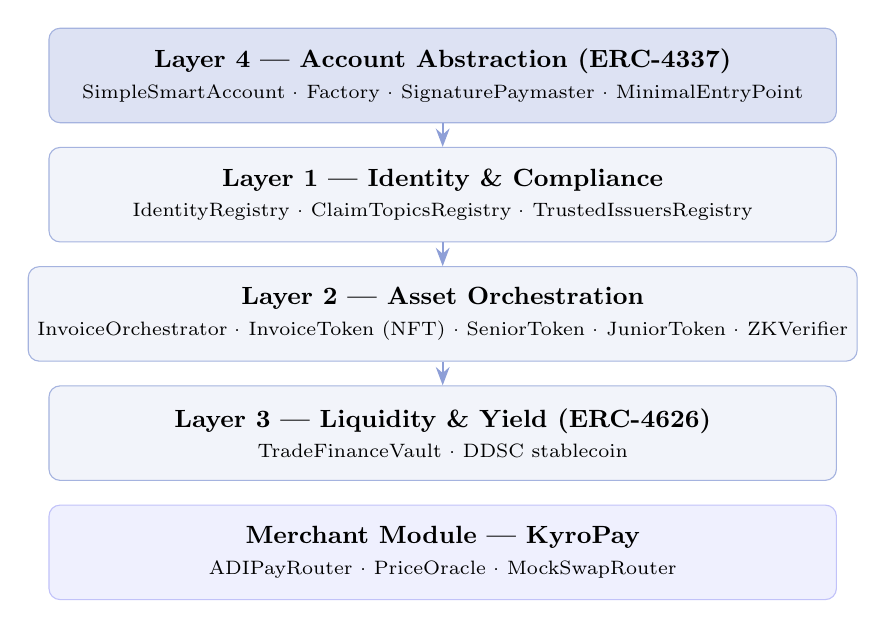
\begin{tikzpicture}[
  layer/.style={
    rectangle, rounded corners=4pt,
    minimum width=10cm, minimum height=1.2cm,
    draw=kyroBlue!40, fill=kyroBlue!6,
    align=center, font=\small\bfseries
  },
  label/.style={font=\tiny\color{kyroGray}, align=center},
  >=Stealth
]

\node[layer, fill=kyroBlue!15] (aa)
  {Layer 4 — Account Abstraction (ERC-4337)\\
   \normalfont\scriptsize SimpleSmartAccount · Factory · SignaturePaymaster · MinimalEntryPoint};

\node[layer, below=0.3cm of aa] (identity)
  {Layer 1 — Identity \& Compliance\\
   \normalfont\scriptsize IdentityRegistry · ClaimTopicsRegistry · TrustedIssuersRegistry};

\node[layer, below=0.3cm of identity] (asset)
  {Layer 2 — Asset Orchestration\\
   \normalfont\scriptsize InvoiceOrchestrator · InvoiceToken (NFT) · SeniorToken · JuniorToken · ZKVerifier};

\node[layer, below=0.3cm of asset] (vault)
  {Layer 3 — Liquidity \& Yield (ERC-4626)\\
   \normalfont\scriptsize TradeFinanceVault · DDSC stablecoin};

\node[layer, below=0.3cm of vault, fill=kyroAccent!10, draw=kyroAccent!40] (merchant)
  {Merchant Module — KyroPay\\
   \normalfont\scriptsize ADIPayRouter · PriceOracle · MockSwapRouter};

\draw[->, thick, color=kyroBlue!50] (aa.south) -- (identity.north);
\draw[->, thick, color=kyroBlue!50] (identity.south) -- (asset.north);
\draw[->, thick, color=kyroBlue!50] (asset.south) -- (vault.north);

\end{tikzpicture}
\caption{Kyro system layers and their dependencies.}
\end{figure}

\noindent The following sections describe each layer in detail.

\subsection{Key Protocol Parameters}

\begin{table}[H]
\centering
\begin{tabularx}{\textwidth}{lX}
\toprule
\textbf{Parameter} & \textbf{Value} \\
\midrule
Network          & ADI Testnet, Chain ID 99999 \\
Senior tranche   & 80\% of invoice face value (\texttt{SENIOR\_BPS = 8000}) \\
Junior tranche   & 20\% of invoice face value (\texttt{JUNIOR\_BPS = 2000}) \\
Senior yield target & 6\% annualized \\
Stablecoin       & DDSC (UAE Dirham-backed, 1 DDSC $\approx$ 1 AED) \\
Vault standard   & ERC-4626 \\
Invoice token    & ERC-721 (non-fungible, one per invoice) \\
Tranche tokens   & ERC-20 (fungible S-DEBT and J-DEBT) \\
AA standard      & ERC-4337 v0.7 \\
Max merchant fee & 200 bps (2\%) \\
\bottomrule
\end{tabularx}
\caption{Kyro protocol parameters.}
\end{table}

% ══════════════════════════════════════════════════════════════════════════════
\section{Layer 1 — Identity \& Compliance}
% ══════════════════════════════════════════════════════════════════════════════

\subsection{Purpose}

Kyro is designed for regulated markets. Every participant — SME, investor, merchant, counterparty
— must be verified before interacting with any protocol asset. Layer 1 implements this requirement
entirely on-chain so that compliance cannot be circumvented by any application-layer action.

\subsection{Contracts}

\subsubsection{IdentityRegistry}

\texttt{IdentityRegistry} is the central source of truth for participant eligibility.
Each registered address is mapped to an \texttt{IdentityRecord}:

\begin{lstlisting}[caption={IdentityRecord data structure}]
struct IdentityRecord {
    bool    registered;    // has an operator enrolled this address?
    bool    kycApproved;   // has a compliance agent approved KYC?
    bytes2  country;       // ISO 3166-1 alpha-2 country code
}
\end{lstlisting}

\noindent Two roles govern the registry:

\begin{itemize}[leftmargin=2em]
  \item \texttt{ADMIN\_ROLE} — deploys and configures the registry; grants/revokes other roles.
  \item \texttt{COMPLIANCE\_AGENT\_ROLE} — registers addresses and manages KYC status.
\end{itemize}

\noindent The external view function \texttt{isVerified(address)} returns \texttt{true} only
when both \texttt{registered} and \texttt{kycApproved} are \texttt{true}.
This function is called by every restricted token before allowing a transfer.

\subsubsection{ClaimTopicsRegistry}

Manages a list of integer claim topics that issuers may attest to (e.g., \texttt{1 = KYC},
\texttt{2 = accredited investor}). Currently one topic is active. The registry is designed
to be extensible for future jurisdiction-specific compliance schemas.

\subsubsection{TrustedIssuersRegistry}

Maintains the set of addresses permitted to issue identity claims. This supports multi-issuer
compliance regimes where different KYC providers operate in different jurisdictions.

\subsection{Enforcement Mechanism}

Compliance checks are embedded inside the \texttt{\_update()} internal hook of every
transfer-restricted ERC-20 and ERC-721 contract. This is the override point exposed by
OpenZeppelin's \texttt{ERC20} and \texttt{ERC721} for all balance-changing operations
(mint, burn, transfer). Pseudo-code:

\begin{lstlisting}[caption={Compliance hook pattern used in SeniorToken and JuniorToken}]
function _update(address from, address to, uint256 amount) internal override {
    // Allow minting (from == 0) and burning (to == 0) freely.
    if (to != address(0)) {
        require(
            identityRegistry.isVerified(to),
            "Recipient is not KYC-verified"
        );
    }
    super._update(from, to, amount);
}
\end{lstlisting}

\noindent Because this hook executes at the EVM level, no application or frontend can bypass it.
An unverified recipient address will cause every transfer to revert unconditionally.

% ══════════════════════════════════════════════════════════════════════════════
\section{Layer 2 — Asset Orchestration}
% ══════════════════════════════════════════════════════════════════════════════

\subsection{Purpose}

Layer 2 implements the factoring engine: it converts an off-chain trade invoice into two
on-chain debt instruments (senior and junior tokens) backed by an NFT representing the legal
claim. It then manages the entire lifecycle of that invoice — from minting through vault purchase,
settlement, or default — in a deterministic, auditable state machine.

\subsection{Contracts}

\subsubsection{InvoiceToken (ERC-721)}

Each invoice is represented by a unique NFT. Token metadata includes:

\begin{lstlisting}[caption={InvoiceToken metadata structure}]
struct InvoiceData {
    uint256 faceValue;      // total DDSC owed
    uint256 dueDate;        // Unix timestamp of repayment deadline
    bytes32 documentHash;   // keccak256 of off-chain invoice document
    address counterparty;   // buyer (obligor) wallet address
    address sme;            // SME (invoice originator) wallet address
}
\end{lstlisting}

\noindent \textbf{Critical design choice:} the NFT is minted directly to the
\texttt{InvoiceOrchestrator} and is never transferred to a user. The NFT acts as an escrow
receipt; only the orchestrator can burn it upon settlement or default. This prevents users
from accidentally trading away their invoice or creating secondary markets in unverified instruments.

\subsubsection{SeniorToken (ERC-20, symbol: S-DEBT)}

Represents the senior tranche: 80\% of the invoice face value. Properties:

\begin{itemize}[leftmargin=2em]
  \item Fixed 6\% yield target, paid from settlement proceeds.
  \item Priority in the repayment waterfall: senior holders are paid first.
  \item Transfers are KYC-gated; only verified institutions may hold S-DEBT.
  \item Minted to and held by the \texttt{InvoiceOrchestrator} until the vault purchases the tranche.
\end{itemize}

\subsubsection{JuniorToken (ERC-20, symbol: J-DEBT)}

Represents the junior tranche: 20\% of the invoice face value. Properties:

\begin{itemize}[leftmargin=2em]
  \item Variable yield: receives whatever remains after senior repayment.
  \item First-loss protection: if the invoice defaults, J-DEBT is burned before S-DEBT takes any loss.
  \item Transfers are KYC-gated.
  \item Minted directly to the SME. This keeps the SME economically aligned — they bear the first
    loss and benefit from any surplus.
\end{itemize}

\subsubsection{InvoiceZKVerifier}

Invoice authenticity is proven without revealing sensitive trade data. A trusted off-chain oracle
inspects the invoice document and signs a compact attestation. The verifier contract checks
the signature:

\begin{lstlisting}[caption={ZK attestation verification (simplified)}]
function verifyInvoice(
    bytes32   invoiceId,
    uint256   faceValue,
    uint256   dueDate,
    bytes32   documentHash,
    bytes calldata zkProof
) external view returns (bool) {
    bytes32 digest = keccak256(abi.encodePacked(
        invoiceId, faceValue, dueDate, documentHash
    ));
    address signer = ECDSA.recover(digest, zkProof);
    return signer == trustedOracle;
}
\end{lstlisting}

\noindent Only the document hash is stored on-chain; the document itself remains off-chain.
Counterparty identities, invoice amounts, and trade terms are never published to the ledger,
satisfying privacy requirements of commercial trade relationships.

\subsubsection{InvoiceOrchestrator}

The orchestrator is the single entry point for all invoice lifecycle operations. It holds MINTER
roles over \texttt{InvoiceToken}, \texttt{SeniorToken}, and \texttt{JuniorToken} and is the
only contract permitted to mint or burn those assets.

\subsection{Invoice State Machine}

An invoice passes through three states:

\begin{figure}[H]
\centering
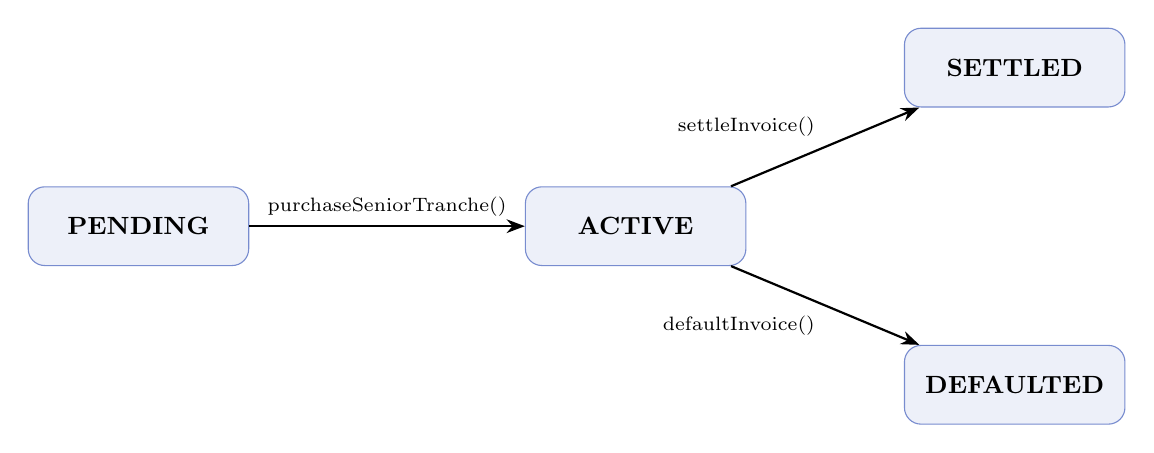
\begin{tikzpicture}[
  state/.style={
    rectangle, rounded corners=6pt,
    minimum width=2.8cm, minimum height=1cm,
    draw=kyroBlue!60, fill=kyroBlue!8,
    align=center, font=\small\bfseries
  },
  >=Stealth, node distance=3.5cm
]
\node[state] (pending) {PENDING};
\node[state, right=of pending] (active)  {ACTIVE};
\node[state, above right=1cm and 2cm of active] (settled)  {SETTLED};
\node[state, below right=1cm and 2cm of active] (defaulted) {DEFAULTED};

\draw[->, thick] (pending)  -- node[above, font=\scriptsize]{purchaseSeniorTranche()} (active);
\draw[->, thick] (active)   -- node[above left,  font=\scriptsize]{settleInvoice()} (settled);
\draw[->, thick] (active)   -- node[below left, font=\scriptsize]{defaultInvoice()} (defaulted);
\end{tikzpicture}
\caption{Invoice lifecycle state machine.}
\end{figure}

\subsection{Invoice Lifecycle: Step-by-Step}

\subsubsection{Step 1 — Minting (\texttt{mintInvoice})}

The SME (or their smart account) calls \texttt{mintInvoice} with:

\begin{itemize}[leftmargin=2em]
  \item \texttt{invoiceId} — a unique \texttt{bytes32} identifier (e.g., \texttt{keccak256(smeAddress, sequenceNumber)}).
  \item \texttt{faceValue} — the total DDSC amount the counterparty owes.
  \item \texttt{dueDate} — the repayment deadline as a Unix timestamp.
  \item \texttt{documentHash} — \texttt{keccak256} of the off-chain invoice document.
  \item \texttt{counterparty} — the buyer's on-chain address.
  \item \texttt{zkProof} — the oracle's ECDSA attestation.
\end{itemize}

\noindent The orchestrator then:

\begin{enumerate}[leftmargin=2em]
  \item Verifies the SME is KYC-approved via \texttt{IdentityRegistry.isVerified()}.
  \item Validates the ZK proof via \texttt{InvoiceZKVerifier.verifyInvoice()}.
  \item Confirms the invoice ID has not been used before.
  \item Mints the \texttt{InvoiceToken} NFT to itself (escrow).
  \item Mints \texttt{SeniorToken} ($= 0.80 \times \texttt{faceValue}$) to itself.
  \item Mints \texttt{JuniorToken} ($= 0.20 \times \texttt{faceValue}$) to the SME.
  \item Stores an \texttt{InvoiceRecord} in state as \texttt{PENDING}.
\end{enumerate}

\noindent All six mutations occur in a single atomic transaction; partial state is impossible.

\subsubsection{Step 2 — Vault Purchase (\texttt{purchaseSeniorTranche})}

A permissioned vault operator calls this function, identified by the \texttt{VAULT\_ROLE}:

\begin{enumerate}[leftmargin=2em]
  \item The orchestrator transfers the Senior tokens to the vault.
  \item The vault transfers DDSC equal to the senior face value to the SME.
  \item The invoice state transitions from \texttt{PENDING} to \texttt{ACTIVE}.
\end{enumerate}

\noindent From the SME's perspective: they submitted an invoice and received DDSC within a single
block. No waiting, no underwriting committee, no wire transfer delay.

\subsubsection{Step 3a — Settlement (\texttt{settleInvoice})}

A settlement oracle (holding \texttt{SETTLEMENT\_ORACLE\_ROLE}) calls this when the counterparty
repays:

\begin{enumerate}[leftmargin=2em]
  \item The oracle transfers DDSC (face value + accrued interest) to the orchestrator.
  \item The orchestrator burns the Senior tokens, Junior tokens, and Invoice NFT.
  \item DDSC is forwarded to the vault.
  \item The vault's \texttt{totalAssets()} increases by the interest amount, causing share price to rise.
  \item State transitions to \texttt{SETTLED}.
\end{enumerate}

\subsubsection{Step 3b — Default (\texttt{defaultInvoice})}

If the due date passes without repayment, the settlement oracle triggers default:

\begin{enumerate}[leftmargin=2em]
  \item Junior tokens are burned entirely (first-loss wipeout — zero recovery to SME's junior position).
  \item Senior tokens are burned; any recovered DDSC is forwarded to the vault up to the senior face value.
  \item The Invoice NFT is burned.
  \item State transitions to \texttt{DEFAULTED}.
\end{enumerate}

\noindent The 80/20 tranching ensures the vault (senior position) is protected until losses exceed
20\% of an invoice's face value before principal impairment begins.

% ══════════════════════════════════════════════════════════════════════════════
\section{Layer 3 — Liquidity \& Yield Vault}
% ══════════════════════════════════════════════════════════════════════════════

\subsection{Purpose}

Layer 3 is the interface between institutional capital and the invoice engine. Investors deposit
DDSC, receive vault shares, and earn yield automatically as invoices settle.

\subsection{ERC-4626 Mechanics}

\texttt{TradeFinanceVault} is a standard ERC-4626 tokenized vault. The two core state quantities are:

\begin{align}
  \texttt{totalAssets()} &= \text{DDSC balance} + \text{S-DEBT balance (valued at par)} \label{eq:total}\\
  \texttt{sharePrice}    &= \frac{\texttt{totalAssets()}}{\texttt{totalSupply()}} \label{eq:price}
\end{align}

\noindent Yield accrual is \emph{automatic and passive}: the share price rises whenever
\texttt{totalAssets()} increases. No reward claiming, no epoch processing.

\subsubsection{Lifecycle Accounting}

Table~\ref{tab:accounting} illustrates the vault's accounting through a complete invoice cycle.

\begin{table}[H]
\centering
\begin{tabularx}{\textwidth}{lXXX}
\toprule
\textbf{Event} & \textbf{DDSC Cash} & \textbf{S-DEBT} & \textbf{totalAssets()} \\
\midrule
Initial state (empty)               & 0       & 0     & 0    \\
Investor deposits 1{,}000 DDSC      & 1{,}000 & 0     & 1{,}000 \\
Vault purchases senior tranche (500)& 500     & 500   & 1{,}000 \\
Invoice settles (500 + 30 interest) & 1{,}030 & 0     & 1{,}030 \\
Investor redeems all shares         & 0       & 0     & 0    \\
\textit{Net investor return}        & \multicolumn{3}{l}{\textit{+30 DDSC (3\% on this invoice cycle)}} \\
\bottomrule
\end{tabularx}
\caption{Vault accounting through one complete invoice cycle.}
\label{tab:accounting}
\end{table}

\noindent Notice that when the vault purchases the senior tranche, \texttt{totalAssets()} is
unchanged: DDSC cash decreases by exactly the amount S-DEBT increases (both valued at par).
There is no dilution or artificial inflation of the share price at purchase time.
The share price rises \emph{only} when interest arrives at settlement.

\subsubsection{Compliance in the Vault}

The vault overrides \texttt{\_update()} to enforce KYC on vault share recipients, mirroring the
pattern used in the tranche tokens. Only verified investors may receive or transfer vault shares.
The DDSC stablecoin itself is not restricted (it is the underlying currency), but vault shares —
which represent a regulated investment interest — are fully compliance-gated.

\subsection{Key Vault Functions}

\begin{table}[H]
\centering
\begin{tabularx}{\textwidth}{lX}
\toprule
\textbf{Function} & \textbf{Description} \\
\midrule
\texttt{deposit(assets, receiver)} & Deposit DDSC; receive proportional shares. \\
\texttt{mint(shares, receiver)}    & Specify desired shares; pay equivalent DDSC. \\
\texttt{redeem(shares, receiver, owner)} & Burn shares; receive DDSC at current share price. \\
\texttt{withdraw(assets, receiver, owner)} & Specify DDSC to receive; burn equivalent shares. \\
\texttt{purchaseSeniorTranche(invoiceId)} & Operator-only: swap DDSC for S-DEBT from orchestrator. \\
\texttt{convertToAssets(shares)}   & Preview DDSC value of a given share count. \\
\texttt{convertToShares(assets)}   & Preview share count for a given DDSC amount. \\
\bottomrule
\end{tabularx}
\caption{TradeFinanceVault public interface.}
\end{table}

% ══════════════════════════════════════════════════════════════════════════════
\section{Layer 4 — Account Abstraction}
% ══════════════════════════════════════════════════════════════════════════════

\subsection{Purpose}

SMEs and merchants are not crypto-native. They should not need to acquire native tokens for gas,
manage multiple wallet keys, or understand the difference between EOAs and contract accounts.
Layer 4 uses ERC-4337 Account Abstraction to make protocol interaction indistinguishable from
using a standard web application.

\subsection{ERC-4337 Overview}

ERC-4337 introduces a pseudo-transaction object called a \texttt{UserOperation} (UserOp). Instead
of sending a regular transaction, a user signs a UserOp. A network of off-chain \emph{bundlers}
batch UserOps and submit them to a canonical \texttt{EntryPoint} contract, which validates and
executes them. A \emph{paymaster} contract can optionally cover the gas cost for users.

\subsection{Contracts}

\subsubsection{SimpleSmartAccount (ERC-4337 Account)}

Each SME gets a deterministically addressed smart contract wallet. Properties:

\begin{itemize}[leftmargin=2em]
  \item Owned by a single EOA; validated by ECDSA signature check.
  \item Can execute arbitrary calls and batched calls (for atomic multi-step operations).
  \item Implements \texttt{validateUserOp()} for ERC-4337 v0.7 compliance.
  \item \textbf{Never holds native ADI tokens} — gas is handled by the paymaster.
\end{itemize}

\subsubsection{SimpleSmartAccountFactory}

A CREATE2 deterministic factory. Given an owner EOA address, it computes a predictable smart
account address. This is critical for compliance onboarding: the compliance agent can KYC-register
a smart account address \emph{before} the account is deployed, so the first protocol interaction
(e.g., minting an invoice) succeeds without a separate deployment step.

\subsubsection{MinimalEntryPoint}

A minimal ERC-4337 v0.7 EntryPoint implementation. Coordinates the validate-then-execute
lifecycle for UserOps submitted by bundlers.

\subsubsection{SignaturePaymaster}

Sponsors gas fees for whitelisted UserOps. Flow:

\begin{enumerate}[leftmargin=2em]
  \item The SME constructs and ECDSA-signs a UserOp off-chain.
  \item The bundler submits the UserOp to the EntryPoint.
  \item The EntryPoint calls \texttt{validatePaymasterUserOp()} on the paymaster.
  \item The paymaster verifies the UserOp signature and returns approval.
  \item The EntryPoint deducts gas from the paymaster's staked ETH deposit.
  \item The SME's smart account executes the desired protocol call (e.g., \texttt{mintInvoice}).
\end{enumerate}

\noindent From the SME's perspective: they clicked a button in a web form. No wallet popup for gas,
no token approval for ADI, no network configuration.

\subsection{Batched Execution}

The smart account supports atomic batched calls. For example, a single UserOp can encode:

\begin{enumerate}[leftmargin=2em]
  \item \texttt{DDSC.approve(orchestrator, amount)}
  \item \texttt{InvoiceOrchestrator.mintInvoice(invoiceId, ...)}
\end{enumerate}

\noindent Both calls execute atomically. If the second fails, the approval is also reverted.
This eliminates the dangling-approval attack surface common in multi-step DeFi flows.

% ══════════════════════════════════════════════════════════════════════════════
\section{Merchant Module — KyroPay}
% ══════════════════════════════════════════════════════════════════════════════

\subsection{Purpose}

KyroPay is a fiat-denominated crypto checkout interface for merchants accepting digital asset
payments. It is architecturally independent of the invoice engine — merchants do not need to
interact with the vault or orchestrator — but it shares the same stablecoin (DDSC) and
operates on the same chain.

\subsection{Contracts}

\subsubsection{PriceOracle}

Maintains a mapping from token address to AED (UAE Dirham) exchange rate. Provides:

\begin{lstlisting}[caption={PriceOracle interface}]
// Returns the number of token units needed to pay fiatAmount (in AED).
function fiatToToken(uint256 fiatAmount, address token)
    external view returns (uint256 tokenUnits);
\end{lstlisting}

\noindent The oracle is initialized with fixed rates at deployment and is designed to be
replaced by a Chainlink aggregator or DEX TWAP feed in production.

\subsubsection{MockSwapRouter}

Executes token-to-token swaps at oracle prices. Allows merchants to specify which token they
wish to receive while the customer pays in a different token. For example:

\begin{itemize}[leftmargin=2em]
  \item Customer pays in mADI (native wrapped token).
  \item Merchant receives DDSC (stablecoin).
  \item The router calculates the equivalence via the oracle and executes the swap atomically.
\end{itemize}

\subsubsection{ADIPayRouter}

The single public entry point for merchant checkout:

\begin{lstlisting}[caption={ADIPayRouter.checkout signature}]
function checkout(
    address merchant,
    uint256 fiatAmount,    // AED-denominated price
    address tokenIn,       // token the customer pays with
    address targetToken    // token the merchant receives
) external;
\end{lstlisting}

\noindent Execution flow:

\begin{enumerate}[leftmargin=2em]
  \item Query \texttt{PriceOracle.fiatToToken(fiatAmount, tokenIn)} to determine customer cost.
  \item Transfer \texttt{tokenIn} from customer to router (customer must have pre-approved).
  \item If \texttt{tokenIn == targetToken}, transfer directly to merchant.
  \item Otherwise, call \texttt{MockSwapRouter.swap(tokenIn, targetToken, amount)} to convert,
    then send \texttt{targetToken} to merchant.
  \item Emit \texttt{CheckoutCompleted(merchant, fiatAmount, tokenIn, targetToken, tokensPaid)}.
\end{enumerate}

\subsection{QR Code Checkout}

The merchant frontend generates a QR code encoding the full checkout configuration as a JSON
object: merchant address, fiat amount, accepted tokens, and preferred receive token. A mobile
wallet scans the code and pre-populates the \texttt{checkout()} call. The merchant UI provides
a live oracle preview showing how many tokens the customer will pay before the transaction is sent.

% ══════════════════════════════════════════════════════════════════════════════
\section{Data Flow: End-to-End Invoice Cycle}
% ══════════════════════════════════════════════════════════════════════════════

This section traces a complete invoice from origination to settlement across all four layers.

\begin{enumerate}[leftmargin=2em, label=\textbf{Step \arabic*.}]

  \item \textbf{KYC Onboarding.}
    A compliance agent calls \texttt{IdentityRegistry.registerIdentity(smeAddress, country)},
    then \texttt{IdentityRegistry.updateKycStatus(smeAddress, true)}.
    The SME is now eligible to interact with the protocol.

  \item \textbf{Smart Account Deployment (optional).}
    The SME's frontend calls \texttt{SimpleSmartAccountFactory.createAccount(ownerEOA)}.
    The resulting deterministic address was already KYC-registered in Step~1.

  \item \textbf{Invoice Minting.}
    The SME signs a UserOp containing a call to \texttt{InvoiceOrchestrator.mintInvoice(...)}.
    The \texttt{SignaturePaymaster} sponsors gas. The orchestrator:
    (a) verifies KYC and ZK proof,
    (b) mints the Invoice NFT to escrow,
    (c) mints 80 S-DEBT to itself,
    (d) mints 20 J-DEBT to the SME.

  \item \textbf{Investor Deposit.}
    A KYC-verified institution calls \texttt{TradeFinanceVault.deposit(1000, institutionAddress)}.
    The vault mints 1{,}000 shares (assuming 1:1 initial price). \texttt{totalAssets() = 1000}.

  \item \textbf{Senior Tranche Purchase.}
    The vault operator calls \texttt{TradeFinanceVault.purchaseSeniorTranche(invoiceId)}.
    The vault sends 800 DDSC to the SME and receives 800 S-DEBT from the orchestrator.
    \texttt{totalAssets()} remains 1{,}000; the share price is unchanged.

  \item \textbf{Settlement.}
    The counterparty repays through the settlement oracle channel.
    The oracle calls \texttt{InvoiceOrchestrator.settleInvoice(invoiceId)}.
    848 DDSC (800 principal + 48 interest at 6\%) is forwarded to the vault.
    The vault burns the S-DEBT and receives 848 DDSC.
    \texttt{totalAssets()} rises from 1{,}000 to 1{,}048. Share price becomes 1.048.

  \item \textbf{Redemption.}
    The investor calls \texttt{TradeFinanceVault.redeem(1000, institutionAddress, institutionAddress)}.
    They receive 1{,}048 DDSC — their original principal plus 48 DDSC in yield.

\end{enumerate}

% ══════════════════════════════════════════════════════════════════════════════
\section{Security Considerations}
% ══════════════════════════════════════════════════════════════════════════════

\subsection{Access Control}

All privileged operations are protected by OpenZeppelin \texttt{AccessControl} roles with
no default admin. Role assignment requires the explicit \texttt{ADMIN\_ROLE}. A role matrix is
maintained across all contracts:

\begin{table}[H]
\centering
\begin{tabularx}{\textwidth}{lXl}
\toprule
\textbf{Role} & \textbf{Permitted Actions} & \textbf{Contract} \\
\midrule
\texttt{ADMIN\_ROLE}            & Grant/revoke roles, configure parameters     & All \\
\texttt{COMPLIANCE\_AGENT\_ROLE}& Register identities, update KYC status       & IdentityRegistry \\
\texttt{MINTER\_ROLE}           & Mint/burn Invoice, Senior, Junior tokens     & Token contracts \\
\texttt{VAULT\_ROLE}            & Call purchaseSeniorTranche, settleInvoice    & Orchestrator \\
\texttt{SETTLEMENT\_ORACLE\_ROLE}& Trigger settlement and default               & Orchestrator \\
\texttt{OPERATOR\_ROLE}         & Sponsor UserOps via paymaster                & SignaturePaymaster \\
\bottomrule
\end{tabularx}
\caption{Role matrix across Kyro contracts.}
\end{table}

\subsection{Re-entrancy}

The orchestrator follows the checks-effects-interactions pattern. All state updates
(\texttt{invoiceRecords[id].state = SETTLED}) occur before external calls (token burns,
DDSC transfers). No re-entrancy guard is required beyond this discipline, but OpenZeppelin's
\texttt{ReentrancyGuard} is applied as defense-in-depth on vault deposit and redeem paths.

\subsection{Oracle Risk}

The \texttt{PriceOracle} and ZK attestation oracle are both trusted components in the current
testnet deployment. In production, the price oracle would be replaced by a Chainlink aggregator
with a staleness check, and the ZK attestation would use a decentralized signing committee or
a formally verified proving system. The architecture isolates these risks behind clean interface
boundaries so the upgrade is a one-contract swap.

\subsection{Invoice Uniqueness}

The orchestrator maintains a \texttt{mapping(bytes32 => InvoiceRecord)} and reverts on any
attempt to mint a duplicate \texttt{invoiceId}. Replay attacks using a previously seen ZK proof
are therefore impossible — the proof is tied to a specific \texttt{invoiceId} which can only be
used once.

\subsection{Junior Tranche Alignment}

Allocating 20\% of the face value as a junior token to the SME is a deliberate economic security
mechanism. The SME has a direct financial stake in ensuring their counterparty repays.
A defaulting SME loses their entire junior position. This alignment reduces moral hazard without
requiring off-chain legal recourse in the normal case.

% ══════════════════════════════════════════════════════════════════════════════
\section{Deployment Architecture}
% ══════════════════════════════════════════════════════════════════════════════

Contracts are deployed in six ordered phases using Foundry deployment scripts.
Each phase exports environment variables consumed by the next:

\begin{table}[H]
\centering
\begin{tabularx}{\textwidth}{clX}
\toprule
\textbf{Phase} & \textbf{Script} & \textbf{Deployed Contracts} \\
\midrule
01 & \texttt{01\_DeployIdentity} & MockDDSC, MockADI, ClaimTopicsRegistry, TrustedIssuersRegistry, IdentityRegistry \\
02 & \texttt{02\_DeployAssetLayer} & InvoiceZKVerifier, InvoiceToken, SeniorToken, JuniorToken, InvoiceOrchestrator; grants MINTER roles \\
03 & \texttt{03\_DeployVault} & TradeFinanceVault; wires IdentityRegistry and SeniorToken references \\
04 & \texttt{04\_DeployAA} & MinimalEntryPoint, SimpleSmartAccountFactory, SignaturePaymaster \\
05 & \texttt{05\_DeployMerchant} & PriceOracle, MockSwapRouter, ADIPayRouter; sets initial exchange rates \\
06 & \texttt{06\_Configure} & Cross-contract wiring: VAULT\_ROLE grant, settlement oracle role, final validation \\
\bottomrule
\end{tabularx}
\caption{Six-phase deployment sequence.}
\end{table}

\noindent All scripts are idempotent and emit structured JSON broadcast files compatible with
Foundry's \texttt{forge script} toolchain.

% ══════════════════════════════════════════════════════════════════════════════
\section{Frontend Architecture}
% ══════════════════════════════════════════════════════════════════════════════

The Kyro frontend is a Next.js 14 application using the Viem library for Ethereum interactions.
It exposes four role-specific portals:

\begin{table}[H]
\centering
\begin{tabularx}{\textwidth}{llX}
\toprule
\textbf{Portal} & \textbf{Route} & \textbf{Primary Actions} \\
\midrule
SME      & \texttt{/sme}      & Submit invoice form; view tranche split; track transaction status \\
Investor & \texttt{/investor} & View vault stats; deposit DDSC; redeem shares; monitor share price \\
Merchant & \texttt{/merchant} & Configure checkout (AED amount, tokens); generate QR code; execute checkout \\
Auditor  & \texttt{/auditor}  & Fetch \texttt{InvoiceMinted}, \texttt{InvoiceSettled}, \texttt{InvoiceDefaulted} events from last N blocks \\
\bottomrule
\end{tabularx}
\caption{Frontend portal summary.}
\end{table}

\noindent The auditor portal is read-only and requires no wallet connection, making it accessible
to compliance officers and regulators without on-chain permissions.

% ══════════════════════════════════════════════════════════════════════════════
\section{Conclusion}
% ══════════════════════════════════════════════════════════════════════════════

Kyro demonstrates that institutional-grade trade finance can be implemented entirely on-chain
without sacrificing compliance, privacy, or user experience. The four-layer architecture —
identity, asset orchestration, yield vault, and account abstraction — is modular by design:
each layer can be independently upgraded, audited, and composed with other DeFi protocols.

The protocol achieves several properties simultaneously that are traditionally considered in
tension:

\begin{itemize}[leftmargin=2em]
  \item \textbf{Compliance without centralization.} KYC is enforced on-chain at the token
    transfer level, not off-chain at the application level.
  \item \textbf{Privacy without opacity.} ZK attestation proves invoice validity without
    exposing trade secrets to the public ledger.
  \item \textbf{Yield without complexity.} ERC-4626 mechanics provide mathematically transparent,
    automatically accruing yield without reward-claiming transactions.
  \item \textbf{Simplicity without insecurity.} ERC-4337 account abstraction removes user-facing
    friction while preserving the full cryptographic security model of the underlying chain.
\end{itemize}

\noindent Kyro's architecture is designed to evolve: oracle integrations can be upgraded to
production-grade feeds, the junior/senior split can be parameterized per invoice, and the
identity layer can accommodate multi-issuer, multi-jurisdiction compliance regimes. The
foundations built here provide a path to production-scale real-world asset tokenization on
the ADI Chain.

% ══════════════════════════════════════════════════════════════════════════════
\section*{Glossary}
\addcontentsline{toc}{section}{Glossary}
% ══════════════════════════════════════════════════════════════════════════════

\begin{description}[leftmargin=3em, style=nextline]
  \item[ADI Chain] A purpose-built EVM-compatible blockchain operated by the ADI Foundation,
    used as the settlement layer for Kyro.
  \item[DDSC] Dubai Dirham Stablecoin — a UAE Dirham-pegged ERC-20 token used as the
    denomination currency throughout Kyro.
  \item[ERC-4337] Ethereum account abstraction standard introducing \texttt{UserOperation}
    objects, bundlers, and paymasters.
  \item[ERC-4626] Ethereum tokenized vault standard defining a standard interface for
    yield-bearing asset vaults.
  \item[J-DEBT] Junior Debt Token — the 20\% junior tranche ERC-20 token representing
    first-loss risk and variable yield.
  \item[KYC] Know Your Customer — the regulatory process of verifying participant identity.
  \item[Paymaster] An ERC-4337 contract that sponsors gas costs on behalf of users.
  \item[S-DEBT] Senior Debt Token — the 80\% senior tranche ERC-20 token representing
    priority repayment and fixed 6\% yield target.
  \item[SME] Small and Medium Enterprise — the invoice originator and junior tranche holder.
  \item[Tranche] A slice of structured debt with defined risk and return characteristics.
  \item[UserOperation] A pseudo-transaction object in ERC-4337 signed by a smart account owner
    and executed by the EntryPoint contract.
  \item[ZK Attestation] A zero-knowledge proof (here: ECDSA oracle signature) proving invoice
    validity without revealing the underlying document.
\end{description}

% ══════════════════════════════════════════════════════════════════════════════
\end{document}
